\section{Схема работы инструмента} 

Схема работы инструмента представлена на рис.~3.1.

\begin{figure}[ht]
	\centering
	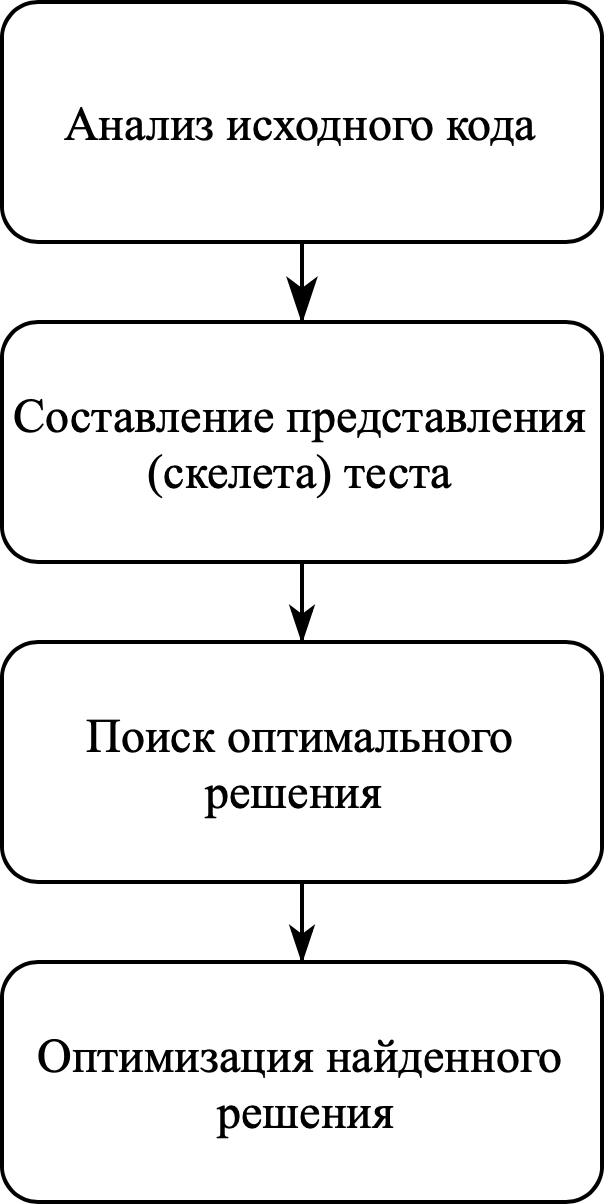
\includegraphics [scale=1.2] {high_level_flow_TR}
	\caption{Схема работы инструмента}
	\label{img:high_level_flow_TR}
\end{figure}

На первой фазе происходит парсинг исходных java файлов. В ходе разбора составляется модель данных, которая содержит следующую информацию:

\begin{itemize}
	\item пакет тестируемого класса;
	\item имя тестируемого класса;
	\item список конструкторов;
	\item список публичных методов с параметрами.
\end{itemize}

В результате получается модель данных, представленная на рис.~3.2.

\begin{figure}[ht]
	\centering
	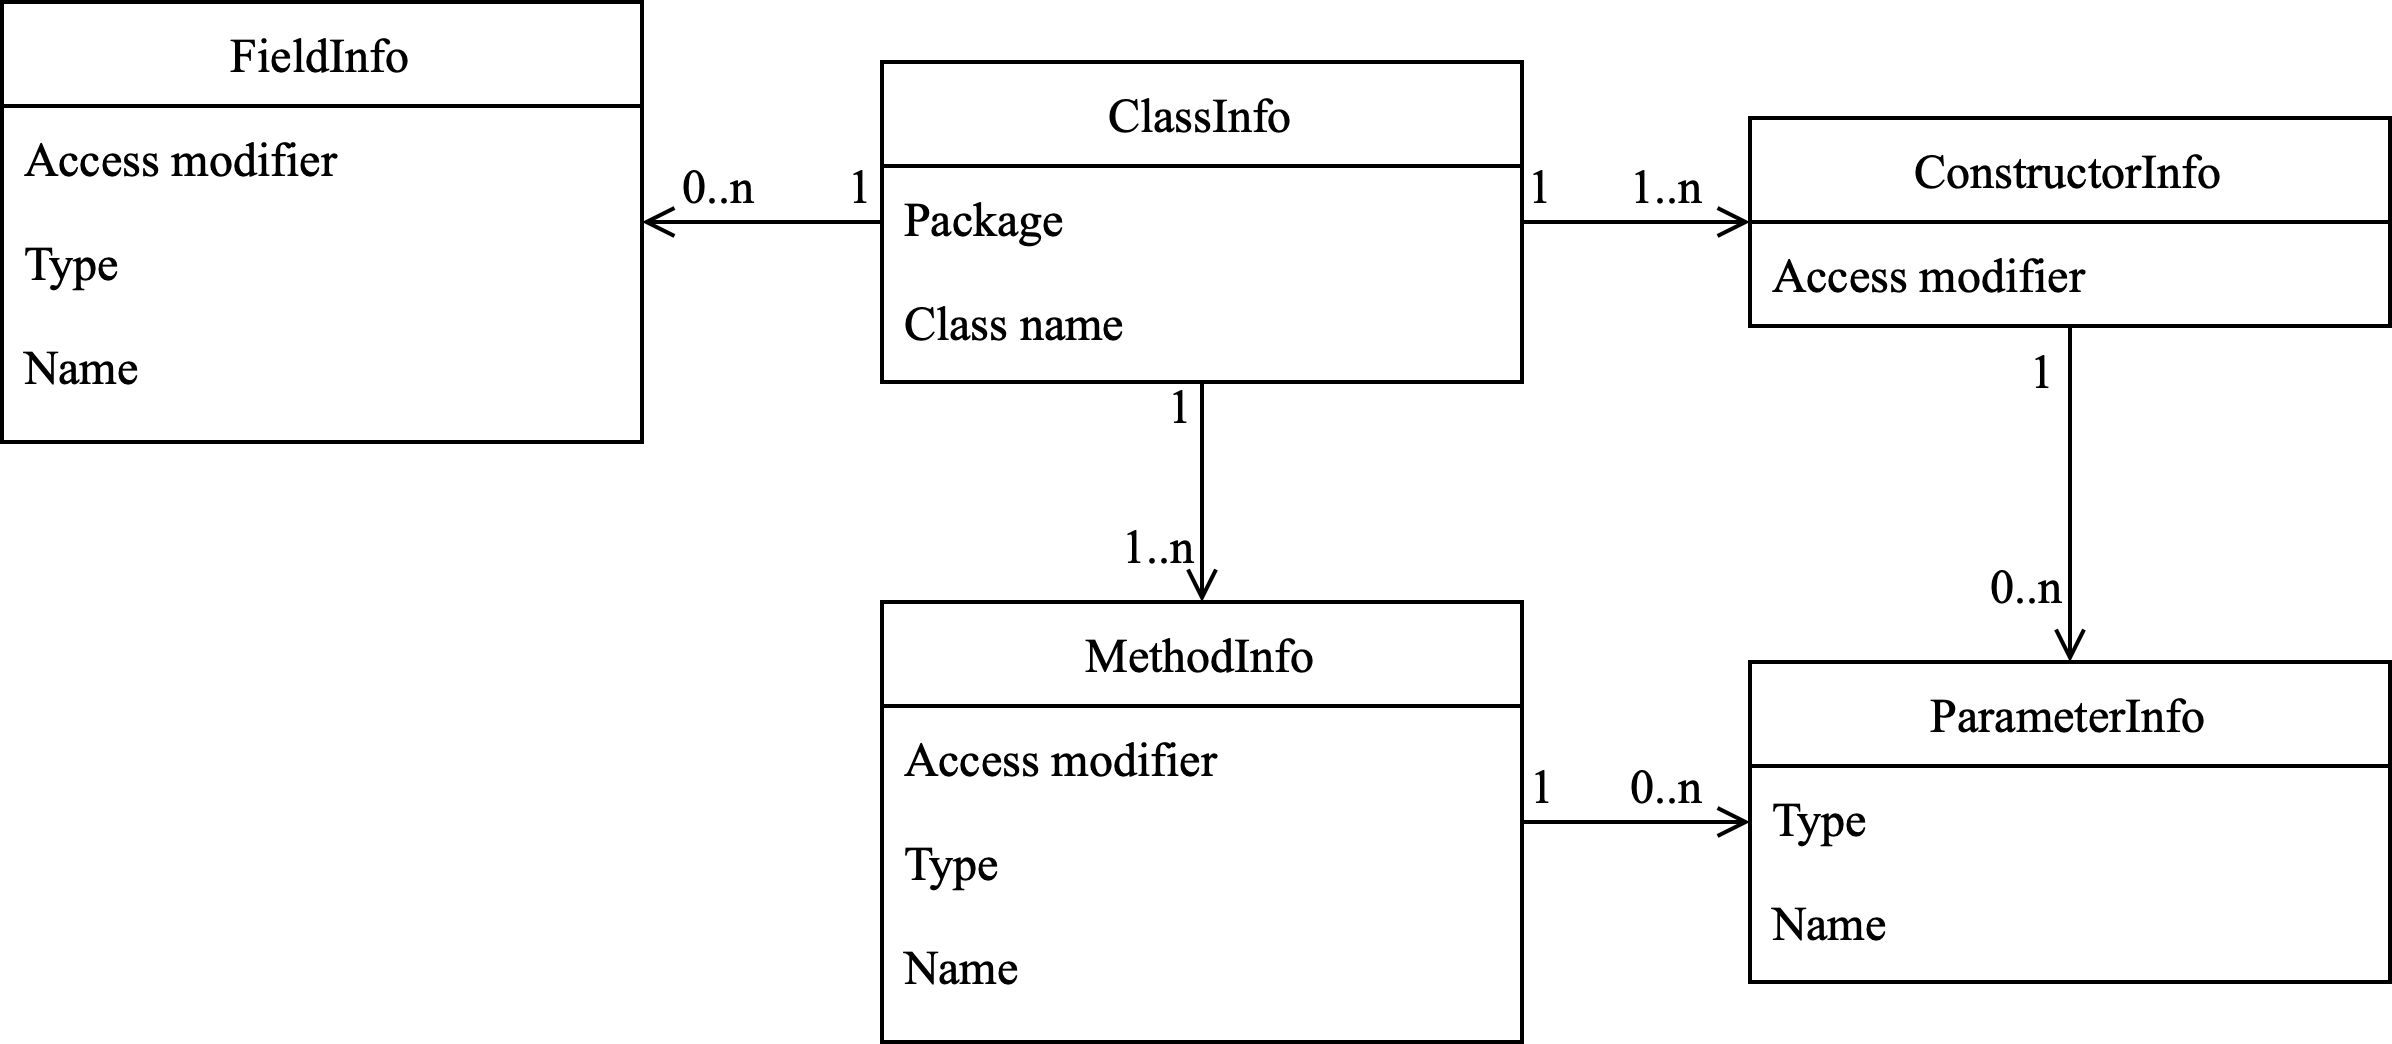
\includegraphics [scale=1] {ClassInfo_diagram_TR}
	\caption{Модель данных}
	\label{img:ClassInfo_diagram_TR}
\end{figure}


После анализа кода происходит создание потенциальных \\ представлений (скелетов) теста. Скелет теста представляет собой прототип кода модульного теста, но без конкретных параметров. На месте параметров находятся специальные заглушки.

Третья фаза~---	поиск оптимального решения.  В качестве реализации поиска был выбран генетический алгоритм.

В конце происходит оптимизация найденного решения. В результате работы алгоритма может получиться тестовый сценарий, который является избыточным. Избыточный тестовый сценарий~--- сценарий, из которого можно убрать часть кода без потери покрытия.


\section{Реализация алгоритма} 

Основным алгоритмом поиска оптимального решения является генетический алгоритм. Визуализация его работы представлена на рис.~3.3.

\begin{figure}[ht]
	\centering
	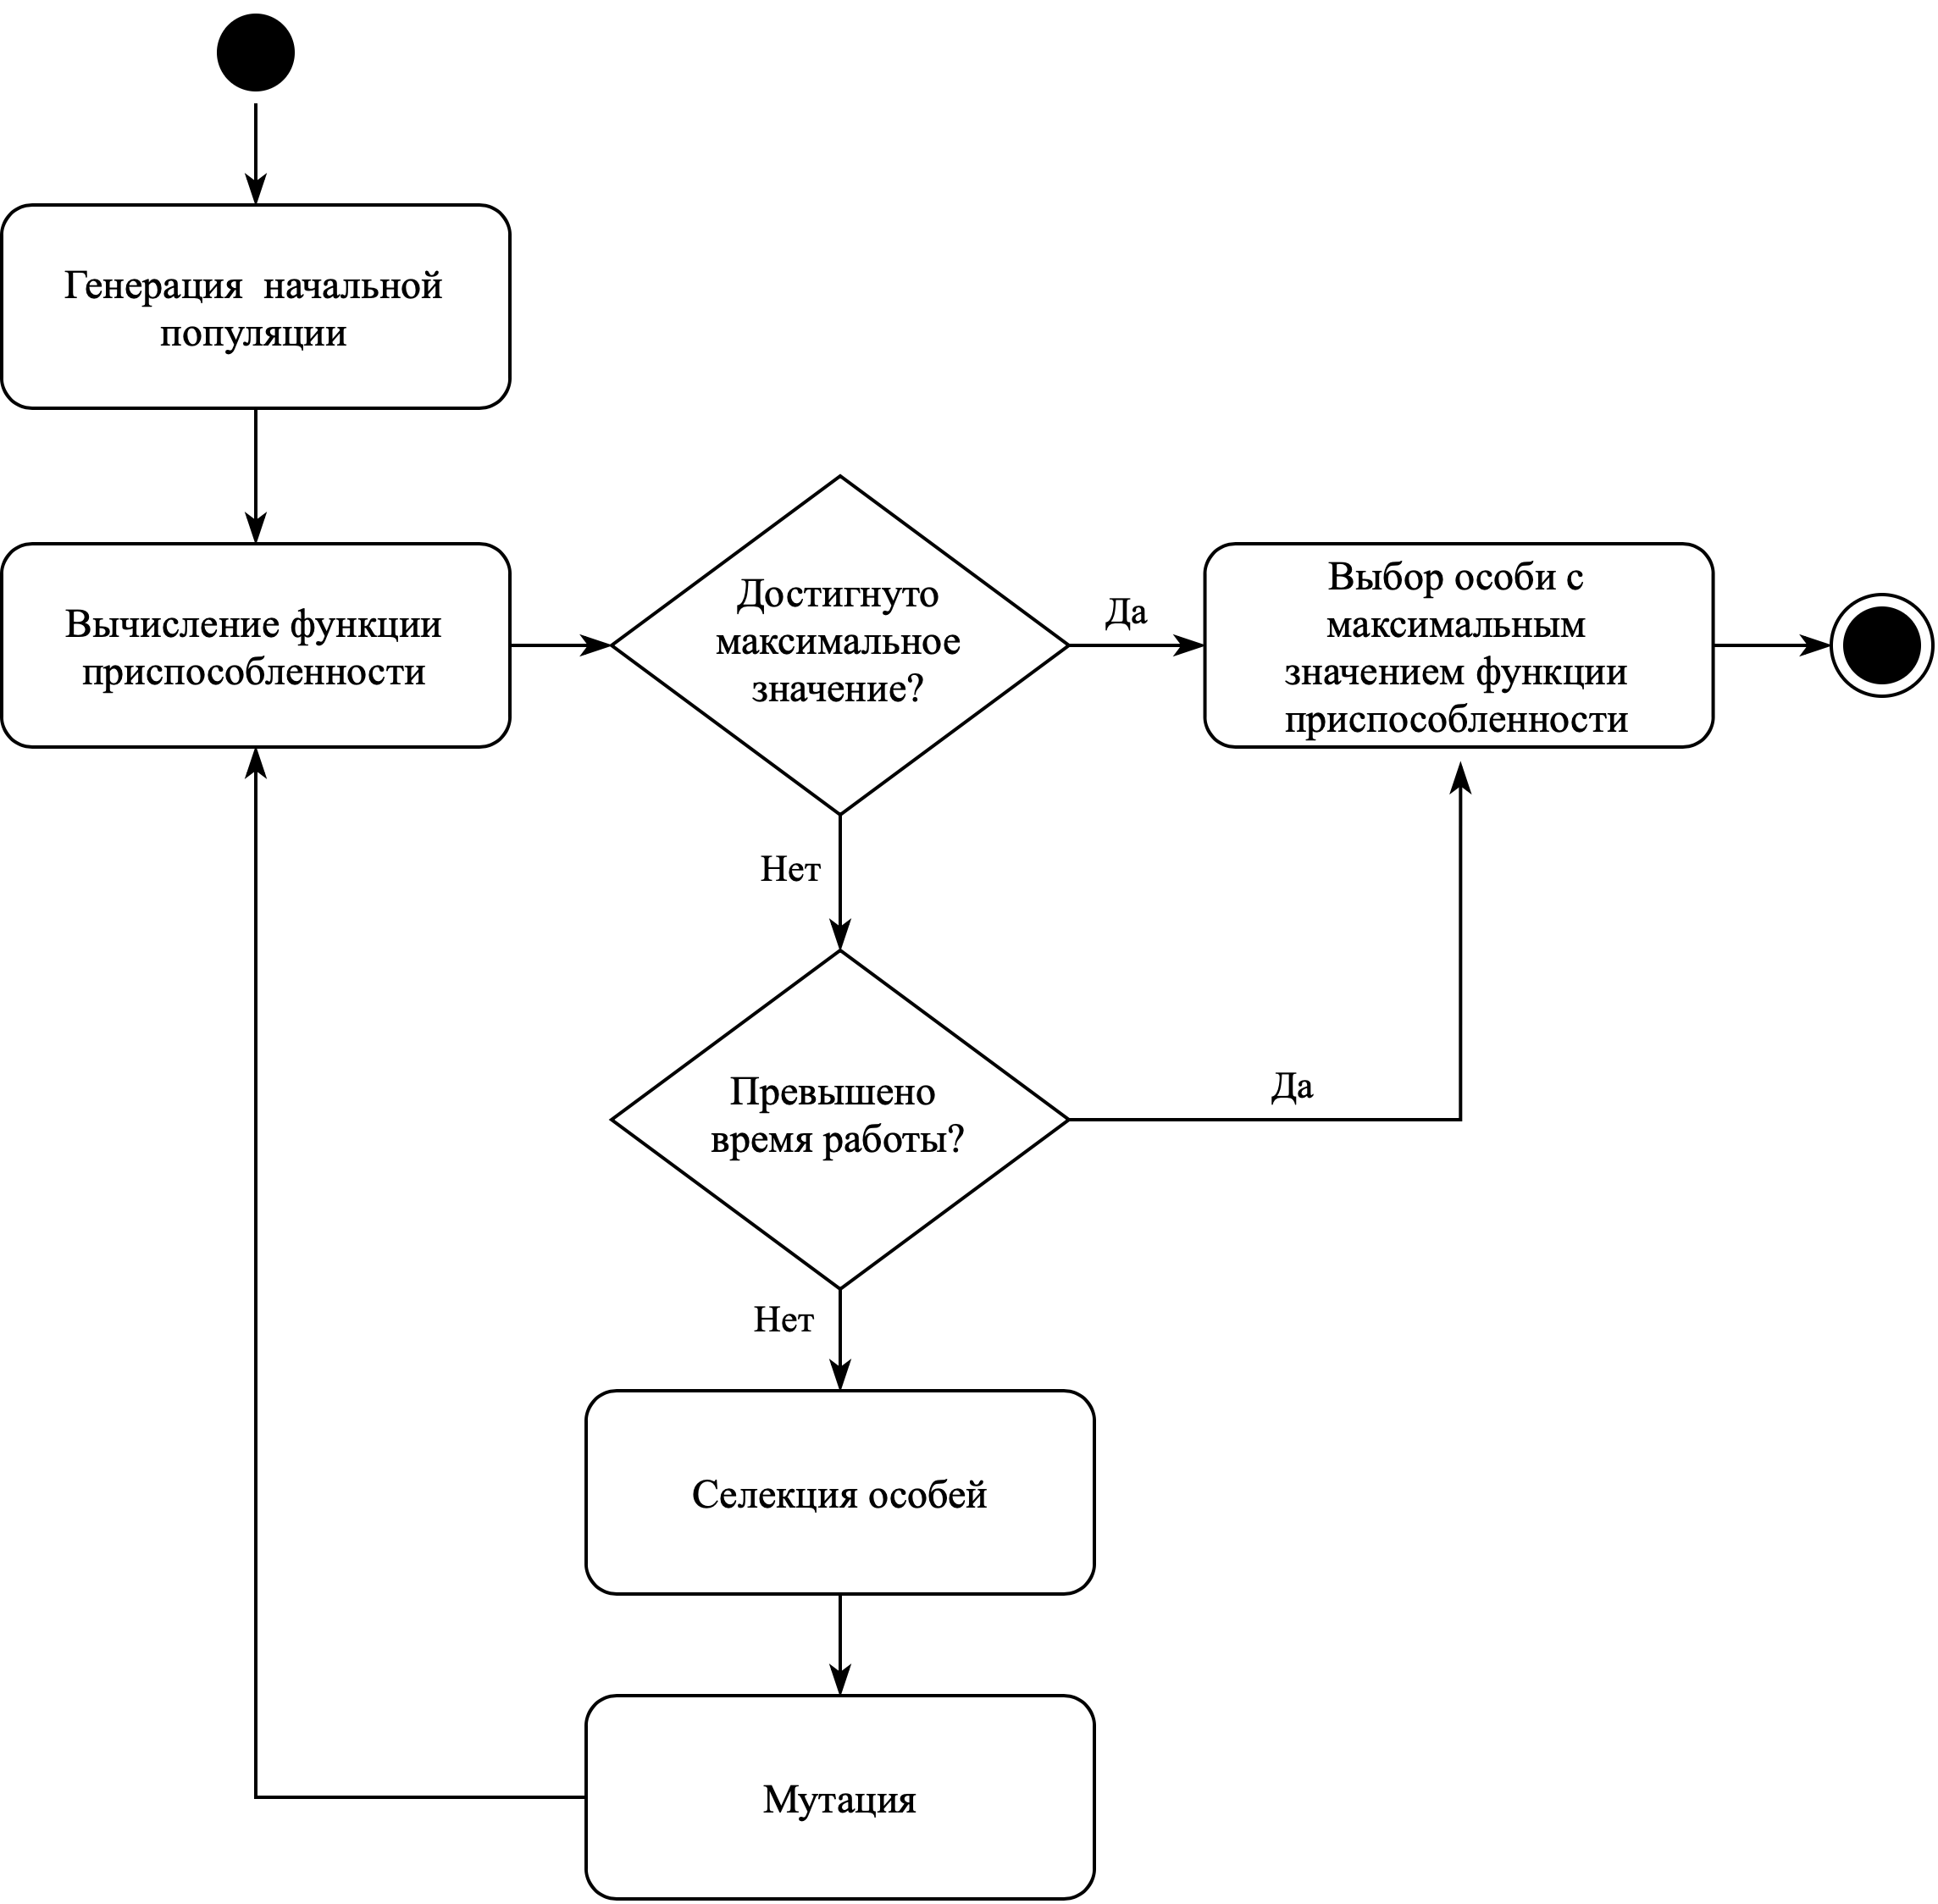
\includegraphics [scale=1] {Genetic_alhorithm_TR}
	\caption{Визуализация работы генетического алгоритма}
	\label{img:Genetic_alhorithm_TR}
\end{figure}

В начале генерируется популяция, которая представляет собой набор скелетов тестов с конкретными параметрами. Затем для каждой особи (конкретный модульный тест) вычисляется функция приспособленности (фитнес функция). Результат функции приспособленности сравнивается с~максимальным (1.0), после чего принимается решение о выходе из алгоритма или продолжении.

Для поиска более удачной комбинации модульных тестов из~популяции выбираются две особи с максимальным значением функции \\ приспособленности (селекция). Выбранные особи скрещиваются, в~результате чего появляются два новых модульных теста, которые объединяют гены (конкретные тестовые методы) особей-предков.

Для избежания попадания в локальные максимумы (ситуация, когда вся популяция сбивается вокруг одно набора генов) на каждой итерации алгоритма используется процесс мутации. Для мутации случайным образом выбираются несколько особей. У выбранных особей запускается процесс мутации, в ходе которого случайный параметр вызова метода заменяется на~другой. Это может быть случайный параметр или мутированный (в случае чисел +1 или -1, в случае строк это замена битов).

\section{Вычисление функции приспособленности}

Функция приспособленности~--- одна из важнейших частей генетического алгоритма. Качество ее работы определяет результат и~скорость работы алгоритма.

Последовательность действий, выполняемая в ходе вычисления функции приспособленности представлена на рис~3.4.

\begin{figure}[ht]
	\centering
	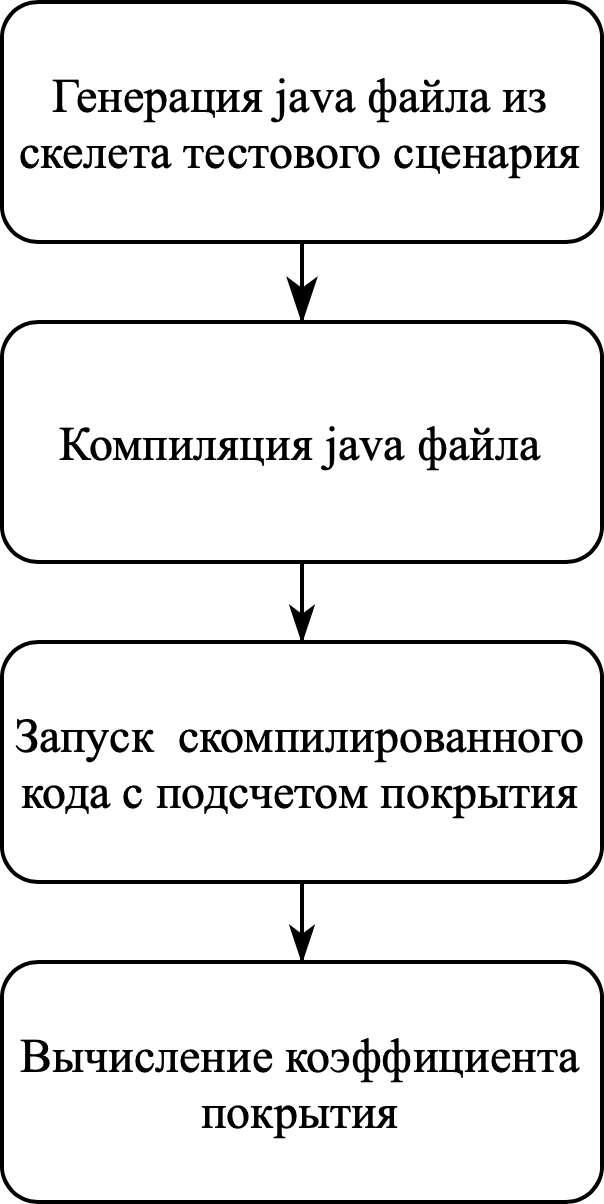
\includegraphics [scale=1.2] {Fitness_function_diagramm_TR}
	\caption{Вычисление функции приспособленности}
	\label{img:Fitness_function_diagramm_TR}
\end{figure}

Для того, что бы оценить качество генерируемого теста, нужно:

\begin{enumerate}
	\item сгенерировать java файл из скелета теста с параметрами;
	\item скомпилировать полученный java файл;
	\item запустить скомпилированный код с подсчетом покрытия по~критерию покрытия ветвей исполнения;
	\item вычислить коэффициент покрытия.
\end{enumerate}

Вычисление коэффициента покрытия происходит по формуле:

\[ \text{коэффициент покрытия} = \frac{\text{количество задействованных ветвей}}{\text{общее количество ветвей}}  \times 100 \% \]

Коэффициент покрытия является результатом работы функции приспособленности.
